\documentclass{amsart}

\input{../preamble_general.tex}

\author{Jalen Chrysos}
\title{Combinatorics Review (With Solutions)}

\begin{document}
	\maketitle 
	
	\noindent \textbf{Problem 1}: Every square on an infinite grid has been colored either red, blue, green, purple, pink, or black. Show that there is a rectangle whose four corners have the same color.\\
	
	\textbf{Solution}: In a row of 7 squares, at least two are the same color, by Pigeonhole principle. And there are only $6^7$ possible color sequences in a row of 7, so in $6^7+1$ rows, at least two have the same sequence of colors, by Pigeonhole principle. If $c$ is a color appearing twice in each of these rows, then between them there is a rectangle with all four corners colored $c$.\\
	
	\noindent \textbf{Problem 2}: Show that any $2^n\times 2^n$ grid, with a square removed, can be tiled by $L$-shaped triominoes:
	
	\begin{figure}[h]
		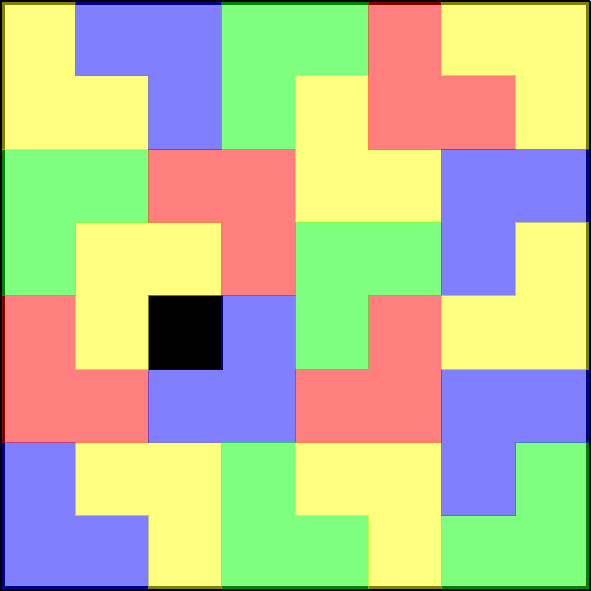
\includegraphics[width=4cm]{./Asymptote_Figs/Lshape.pdf}
	\end{figure}
	
	\textbf{Solution}: We argue by induction. The case $n=1$ is clear; whichever square is removed, the remaining squares can be covered by a single $L$. Now suppose that the statement is true of $n$, and we will prove it for $n+1$: a $2^{n+1}\times 2^{n+1}$ board can be split into four quadrants of sizes $2^n\times 2^n$. One of these has a square removed, and can thus be tiled by $L$-shapes by the inductive hypothesis. Next, we place an $L$-shape in the middle of the $2^{n+1}\times 2^{n+1}$ board so that it covers exactly one square in each of the three remaining quadrants. The remaining quadrants now have a square removed, so they can be tiled by $L$-shapes by the inductive hypothesis. Thus, the $2^{n+1}\times 2^{n+1}$ board is tiled.
	
	\begin{figure}[h]
		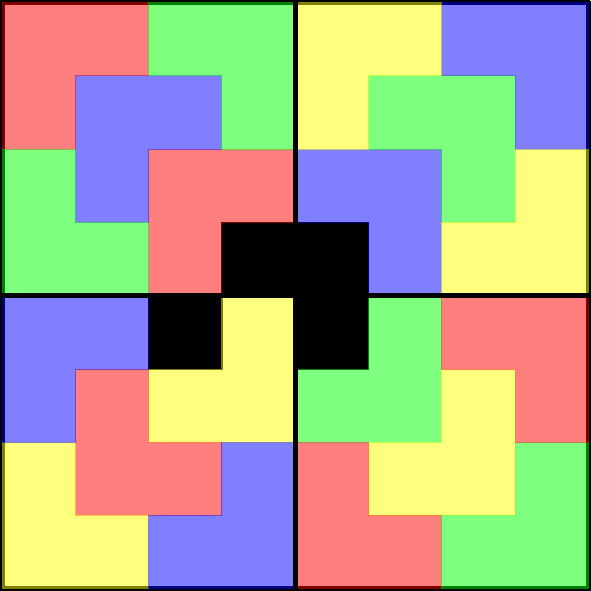
\includegraphics[width=4cm]{./Asymptote_Figs/Lshape2.pdf}
	\end{figure}
	
	\noindent \textbf{Problem 3}: King Blear has 100 daughters and a kingdom of 1000 acres of land. He wants to give each of his daughters an inheritance of some whole number of acres between 0 and 1000. In how many ways can he do this? Assume each acre of land is indistinguishable. You can give your answer in terms of binomial coefficients.\\
	
	\textbf{Solution}: This technique is sometimes called ``stars and bars.'' King blear can place 1000 acre tokens in a row, representing acres of land, and place 99 divider tokens between them, breaking the acres into 100 sections, and give the $k$th section of acres to the $k$th daughter. Any distribution of acres is uniquely expressed by exactly one of these token orderings, so it suffices to count how many different ways he can order the tokens. With acres and dividers both placed in the row, there are 1099 total tokens in the row, and he must choose 99 of them to be dividing tokens, and the number of ways to do this is expressed by the binomial coefficient
	$$
	{1099 \choose 99}.
	$$
	
	\noindent \textbf{Problem 4}: Let $A\subseteq \{1,2,\dots,1000\}$ be a set of size $501$. Show that there exist a pair of distinct elements $x,y\in A$ such that $x|y$ ($x$ divides $y$).\\
	
	\textbf{Solution}: Divide $\{1,2,\dots,1000\}$ into parts $\{m,2m,2^2m,2^3m,\dots\}$ for each odd $m$ between $1$ and $999$, so there are 500 parts (and note that they are disjoint). By Pigeonhole principle, one of these parts contains 2 elements of $A$, and one of these elements must divide the other.\\
	
	%	\noindent \textbf{Problem}: A class of $n$ students all forget to write their student ID number on their quizzes, so they are handed back randomly. Let $A_n$ be the number of ways to hand the quizzes back so that \textit{no student receives their own quiz}. 
	%	\begin{enumerate}[(a)]
		%		\item Find an recursive expression for $A_n$ (that is, find a formula for $A_n$ in terms of earlier entries in the sequence).
		%		\item Show that 
		%		$$
		%		A_n = n! \bigg(\sum_{k=0}^n \frac{(-1)^k}{k!}\bigg)
		%		$$
		%		\item (optional) As $n\to\infty$, the probability that no student receives their own quiz converges to a limit. What is that limit?\\
		%	\end{enumerate}
	%	
	%	\textbf{Solution}: \\
	
	%	(a): Let the students be numbered $1,2,\dots,n$. $A_n$ can also be viewed as the number of directed graphs on $n$ vertices where every vertex has out-degree 1 (and doesn't point to itself). Suppose wlog that $1\mapsto 2$, though there are $n-1$ choices. There are two cases: if $2\mapsto 1$, then t\\
	%	
	%	(b): 
	
	\noindent \textbf{Problem 5}: For $n\geq 5$, show that 
	$$
	{5 \choose 5} + {6 \choose 5} + \cdots + {n\choose 5} = {n+1\choose 6}.
	$$
	
	\textbf{Solution}: We use induction. For $n=5$ the claim is just saying ${5\choose 5} = {6\choose 6}$, which is true. Now suppose that it is true for $n$, then
	$$
	{5 \choose 5} + {6 \choose 5} + \cdots + {n\choose 5} + {n+1\choose 5} = {n+1 \choose 6} + {n+1 \choose 5}.
	$$
	So now we need to show ${n+1 \choose 6} + {n+1\choose 5} = {n+2\choose 6}$, which can be shown as follows: when choosing 6 numbers from among $\{1,2,\dots,n+2\}$, either they're all below $n+2$, or 5 are below $n+2$ and the last is $n+2$. There are ${n+1\choose 6}$ ways to choose them in the former way, and ${n+1\choose 5}$ in the latter. This could also be shown by looking at Pascal's triangle.\\
	
	\noindent \textbf{Problem 6}: An ant stands on one vertex of a cube. Every day the ant randomly moves to one of the three vertices adjacent to its current vertex. The vertex opposite to where the ant starts is its goal.
	
	\begin{enumerate}[(a)]
		\item Find the probability that after five days' travel, the ant is on the goal vertex.
		\item Find the expected number of days that it will take for the ant to reach the goal.
	\end{enumerate}
	
	\begin{figure}[h]
		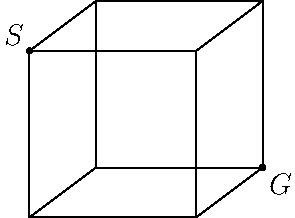
\includegraphics[width=4cm]{./Asymptote_Figs/Ant1.pdf}
	\end{figure}
	
	\textbf{Solution}: \\
	
	(a): One way to do this is count the number of paths to get to each vertex on each day. This can be done recursively: the number of length $n$ paths ending at $v$ is equal to the number of length $n-1$ paths ending at neighbors of $v$, since each of these paths can be extended in a unique way to $v$. Using this fact, we can calculate the number of paths to each vertex on each day:
	
	\begin{figure}[h]
		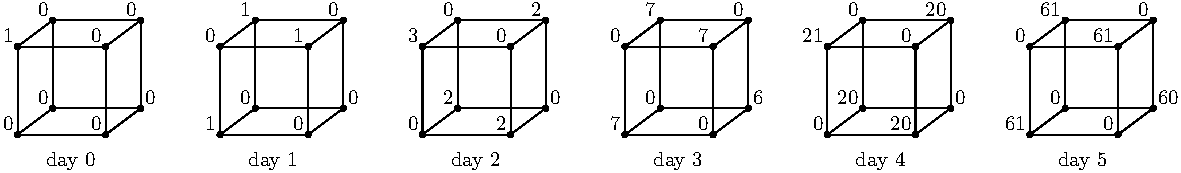
\includegraphics[width=15cm]{./Asymptote_Figs/Ant3.pdf}
	\end{figure}
	
	So the answer is $60/243 = 20/81$.\\
	
	(b): By symmetry, we can divide the cube into parts $A,B,C,D$ by their distance to the goal. 
	
	\begin{figure}[h]
		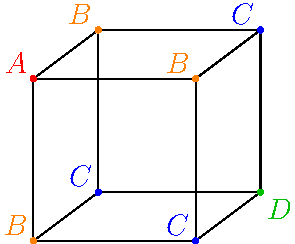
\includegraphics[width=4cm]{./Asymptote_Figs/Ant2.pdf}
	\end{figure}
	
	Let $\E(A)$ be the expected number of days to reach the goal starting at vertex $A$, $\E(B)$ the expected number of days starting at any vertex of $B$ (they are all symmetric), and similarly $\E(C)$.
	
	These values can be related: from $A$, after 1 day of travel the ant reaches $B$, from which the expected number of days is $\E(B)$. From $B$, after 1 day of travel, the ant returns to $A$ $\tfrac13$ of the time, and goes to $C$ $\tfrac23$ of the time. And similarly when starting at $C$, after 1 day of travel, the ant returns to $B$ $\tfrac23$ of the time, and goes to $D$ $\tfrac13$ of the time. So we have the following three relations between $\E(A),\E(B),\E(C)$:
	\begin{align*}
		\E(A) &= 1 + \E(B)\\
		\E(B) &= 1 + \tfrac13 \E(A) + \tfrac23 \E(C)\\
		\E(C) &= 1 + \tfrac23 \E(B) + \tfrac13(0)
	\end{align*}
	Solving this system of equations yields $\E(A)=10,\E(B)=9,\E(C)=7$. So the answer is 10 days.
\end{document}